\section*{Appendix}

\subsection{Constraints of successive MPC problems}
\label{sec:inclusions statement}
We are now ready to state and prove a key lemma regarding the evolution of the state, error and input sets between MPC optimization problems. 
This lemma will be key to proving recursive feasibility of the MPC controller, since it allows us to show that the constraint sets of one problem, at time $k$, are appropriate supersets of the constraint sets of the next problem, at time $k+1$. 

\begin{lemma}
	\label{lem:set inclusions}
	Let $\oa{X}_{k+j|k}$ be the $j$-step outer-approximate reach set computed at time $k$ by a reachability tool as described in Sec. \ref{sec:x reach}.
	
	Let $\What_{k+j|k}$ be the set defined in \eqref{eq:What}.
	
	Let $\tE_{k+j|k}$ be the error set computed using \eqref{eq:H}, \eqref{eq:tildeE} by substituting $E \leftarrow \tE_{k|k}$.
	
	Let $\ua{V}_{k+j|k} = \ua{V}(\oa{X}_{k+j|k})$ and $\oa{V}_{k+j|k} = \oa{V}(\oa{X}_{k+j|k})$ 

Then the following hold for all $k \geq 0, ,j \geq 1$:
\begin{enumerate}
	\item $\oa{X}_{k+1+j|k+1} \subseteq \oa{X}_{k+j+1|k}$
	\label{set:X}
	\item $\tE_{k+1+j|k+1} \subseteq \tE_{k+j+1|k}$
	\label{set:tE}
	\item $\What_{k+1+j|k+1} \subseteq \What_{k+j+1|k}$
	\label{set:What}
	\item $\oa{V}_{k+1+j|k+1} \subseteq \oa{V}_{k+j+1|k}$
	\label{set:oaV}
	\item $\ua{V}_{k+1+j|k+1} \supseteq \ua{V}_{k+j+1|k}$ (note the change in inclusion direction)
	\label{set:uaV}		
\end{enumerate} 
\end{lemma} 

\begin{proof}
	
\ref{set:X}) 
Fix an arbitrary $k$. We prove this by induction on $j \geq 1$.

\underline{Base case: $j=1$}. By construction, $\hx_{k+1} \in \RT{\Xset{k}{k}} \oplus E$.
Therefore at time $k+1$, when setting up the problem $\mathbb{P}_{k+1}(\hat{z}_{k+1})$, the algorithm will first compute
$\Xset{k+1}{k+1} = \hx_{k+1} \oplus (-E)  \subset \RT{\Xset{k}{k}} \oplus E \oplus (-E) = \oaXset{k+1}{k}$.
Also 
$\oaXset{k+2}{k+1} = \RT{\Xset{k+1}{k+1}} \oplus E \oplus(-E) \subset  \RT{\oaXset{k+1}{k}} \oplus E \oplus(-E) = \oaXset{k+2}{k}$.

\underline{Induction step: $j > 1$}.
By definition, $\oaXset{k+1+j}{k+1} = \RT{\oaXset{k+1+j-1}{k+1}} \oplus E \oplus (-E) \subset  \RT{\oaXset{k+j}{k}} \oplus E \oplus (-E)$ (by the induction hypothesis). This last set equals $\oaXset{k+j+1}{k}$ by definition.

\ref{set:tE}) 	By \ref{set:X}) 
 we have that 
 $ \min_{x \in \oa{X}_{k+j+1|k}, e \in E} M_{i\ell}(x)e(\ell) \leq \min_{x \in \oa{X}_{k+1+j|k+1}, e \in E} M_{i\ell}(x)e(\ell)$ and that 
 $\max_{x \in \oa{X}_{k+j+1|k}, e \in E} M_{i\ell}(x)e(\ell) \leq \max_{x \in \oa{X}_{k+1+j|k+1}, e \in E} M_{i\ell}(x)e(\ell)$
 which yields the desired result.
 
 \ref{set:What}) This is immediate from the definition \eqref{eq:What} and \ref{set:tE}).
 
 \ref{set:oaV}) and \ref{set:uaV}) These are immediate from \eqref{eq:V inclusions}.
 
	\end{proof}


\subsection{Proof of Theorem \ref{th:robust_feas}}
\label{sec:proof of thm 1}
We will prove the Theorem by recursion by showing that if at time step $k$, the problem $\mathbb{P}_{k}(\hat{z}_k)$ is feasible and the feasible control input $v_k = v^{*}_{k|k}$ is applied, then $v_k$ is admissible (meets the system constraints) and at time $k+1$, $z_{k+1}$ is inside $Z$ and also $\mathbb{P}_{k+1}(\hat{z}_{k+1})$ is feasible for all disturbances. By recursion then, if we have feasibility at step $k=k_0$, we have robust constraint satisfaction and feasibility at time step $k_0+1$ and so on for all $k>k_0$. 

To begin, let $\mathbb{P}_{k}(\hat{z}_k)$ be feasible, then it has a feasible solution $(\lbrace z^{*}_{k+j|k}\rbrace_{j=0}^{N+1}, \, \lbrace v^{*}_{k+j|k}\rbrace_{j=0}^{N} )$ that satisfies all the constraints of the Robust MPC. 
Now let's construct a feasible candidate solution for $\mathbb{P}_{k+1}(\hat{z}_{k+1})$ at the next time step by shifting the above solution one-step forward. 
Consider the candidate solution:

\begin{subequations}
\begin{align}
\label{eq:candidate}
\nz_{k+j+1|k+1} &= z^{*}_{k+j+1|k} + L_j\hat{w}_{k+1}, \, \forall j \in [0:N]\\
\nz_{k+N+2|k+1}&= A\nz_{k+N+1|k+1} + B\bar{v}_{k+N+1|k+1} \\
\bar{v}_{k+j+1|k+1}&=v^{*}_{k+j+1|k} + KL_j\hat{w}_{k+1}, \, \forall j \in [0:N-1]\\
\bar{v}_{k+N+1|k+1}&=K\nz_{k+N+1|k+1} 
\end{align}
\end{subequations}

First we will show that the input and state constraints are satisfied by $v_k$ and $\nz_{k+1}$, then prove feasibility of the above candidate solution for $\mathbb{P}_{k+1}(\hat{z}_{k+1})$.

\textit{Validity of input and next state:}
The next state is:
\begin{eqnarray}
\label{eq:z_next}
z_{k+1} &= &Az_k + Bv_k + w_k \nonumber
\\
&=& A(\hat{z}_k-\tilde{e}_k)+Bv^{*}_{k|k}+w_k \nonumber \\
 &=& A\hat{z}_k+Bv^{*}_{k|k}-\tilde{e}_{k+1}+(w_k+\tilde{e}_{k+1}-A\tilde{e}_k) \nonumber \\
  &=& Az^{*}_{k|k} +Bv^{*}_{k|k}-\tilde{e}_{k+1}+  \hw_{k+1} \nonumber\\
  & \;& \quad (\Pk{k} \text{ initialization}) \nonumber \\
&= &z^{*}_{k+1|k} - \tilde{e}_{k+1} + \hat{w}_{k+1} 
\end{eqnarray}

By feasibility of the solution at time $k$,
\begin{equation*}
z^{*}_{k+1|k} \in\nomZset{k+1}{k} = Z \ominus (-\tilde{E}_{k+1|k}) \ominus L_0\What_{k+1|k}
\end{equation*}

Therefore, $z_{k+1} \in Z$ and so $x_{k+1} \in X$.
%By definition, $\tilde{e}_{k+1} \in \tilde{E}_{k+1|k}$ and $\hat{w}_{k+1} \in  \What_{k+1|k}$. Using this fact, definition of Pontraygin difference and Eq. \ref{eq:z_next} (also remember, $L_0 = \mathbb{I}$), we have that:

Moreover, by the feasibility of $v^{*}_{k|k}$ for $\mathbb{P}_{k}(\hat{z}_k)$ and by the definition of $\underline{V}_{k|k}$,
$v_k = v^{*}_{k|k} \in \underline{V}_{k|k}$, which implies that $u_k \in U$.

Hence, if $\mathbb{P}_{k}(\hat{z}_k)$ is feasible, then the applied input at time step $k$ and the resulting next state $z_{k+1}$ (and hence $x_{k+1}$) are admissible under all possible disturbances. 
The next part of the proof will focus on showing that the candidate solution of Eq. \eqref{eq:candidate} is indeed feasible for $\Pk{k+1}$ by proving that it meets all the constraints.

\textit{Initial Condition:} Recall from \eqref{eq:dynamics_estimate} that $\hat{z}_{k+1} = A\hat{z}_k + Bv_k + \hat{w}_{k+1}$.
Also by the construction of the candidate solution,
\begin{subequations}
\begin{align}
\nz_{k+1|k+1} &= z^{*}_{k+1|k} + L_0 \hat{w}_{k+1} \nonumber \\
&= Az^{*}_{k|k} + Bv^{*}_{k|k} + \hat{w}_{k+1}
\end{align}
\end{subequations}

Since $z^{*}_{k|k}=\hat{z}_k$ and $v^{*}_{k|k} = v_k$, by the two equations above, we have
\begin{equation}
\nz_{k+1|k+1} = \hat{z}_{k+1}
\end{equation}

Hence, the candidate solution does indeed satisfy the initial condition for $\Pk{k+1}$.
Next we show that the candidate solution satisfies the nominal dynamics:

\textit{ Nominal Dynamics:} For $0\leq j<N$,we have:
\begin{eqnarray*}
&& \nz_{k+j+2|k+1} 
\\
&& = z^{*}_{k+j+2|k} + L_{j+1}\hat{w}_{k+1} \\
&& = Az^{*}_{k+j+1}+Bv^{*}_{k+j+1|k} + L_{j+1}\hat{w}_{k+1} \\
&& \text{By the construction of the candidate solution} \nonumber \\
&& = A(\nz_{k+j+1|k+1}-L_j\hat{w}_{k+1}) + B(\bar{v}_{k+j+1|k+1} - KL_j \hat{w}_{k+1}) \nonumber \\
&& \;\; + L_{j+1}\hat{w}_{k+1} \\
&& = A\nz_{k+j+1|k+1} + B\bar{v}_{k+j+1|k+1} -(A+BK)L_j\hat{w}_{k+1} \nonumber \\
&& \;\; + L_{j+1}\hat{w}_{k+1} \\
&& = A\nz_{k+j+1|k+1} + B\bar{v}_{k+j+1|k+1} - L_{j+1}\hat{w}_{k+1} + L_{j+1}\hat{w}_{k+1} \\
&& = A\nz_{k+j+1|k+1} + B\bar{v}_{k+j+1|k+1}
\end{eqnarray*}

For $j=N$, by construction $\nz_{k+N+2|k+1} = A\nz_{k+N+1|k+1} + B\bar{v}_{k+N+1|k+1}$. Hence, the candidate solution does indeed satisfy the nominal dynamics.

\textit{State Constraints:} To show feasibility of the candidate solution w.r.t the state constraints, we need to show that $\nz_{(k+1)+j|k+1}\in \nomZset{k+1+j}{k+1}\, \forall j=0,\dotsc,N$. Re-writing Eq.\ref{eq:Set_constraints} for $\mathbb{P}_{k}(\hat{z}_k)$ for $j=0,\dotsc,N-1$, we have:

\begin{subequations}
\label{eq:redef_Zj}
\begin{align}
& \nomZset{k+j+1}{k} \nonumber
\\
\; \; &= Z \ominus_{i=0}^{j}L_i\What_{k+j+1-i|k} \ominus (-\tilde{E}_{k+j+1|k}) \nonumber \\
 &= Z \ominus L_j \What_{k+1|k} \ominus_{i=1}^{j}L_i\What_{k+j+1-i|k} \ominus (-\tilde{E}_{k+j+1|k}) \nonumber\\
 &= Z \ominus L_j \What_{k+1|k} \ominus_{i=0}^{j-1}L_i\What_{k+j-i|k} \ominus (-\tilde{E}_{k+j+1|k}) \nonumber
\end{align}
\end{subequations}


Also, let us write the state constraints for all $j=0,\dotsc,N$ for the problem at time $k+1$, i.e. for $\mathbb{P}_{k+1}(\hat{z}_{k+1})$:
\begin{equation*}
\label{eq:redef_Zjp1}
\nomZset{(k+1)+j}{k+1} = Z \ominus_{i=0}^{j-1}L_i\What_{k+j-i|k+1} \ominus (-\tilde{E}_{k+1+j|k+1}) \\
\end{equation*}

Remember, by construction of the candidate, we have $\nz_{k+j+1|k+1} = z^{*}_{k+j+1|k} + L_j\hat{w}_{k+1}$.
Also by feasibility of the algorithm at time $k$, we have $z^{*}_{k+j+1|k}\in \nomZset{k+j+1}{k}$, and by definition, $L_j\hat{w}_{k+1} \in L_j\What_{k+1|k}$. 
Therefore by Eq. \eqref{eq:redef_Zj}, we have $\forall j=0,\dotsc,N-1$,
\begin{equation}
\nz_{(k+1)+j|k+1} \in Z \ominus_{i=0}^{j-1}L_i\What_{k+j-i|k} \ominus (-\tilde{E}_{k+j+1|k}) \\
\end{equation}
Using points 2) and 3) from Lemma \ref{lem:set inclusions},
\begin{eqnarray*}
&&Z \ominus_{i=0}^{j-1}L_i\What_{k+j-i|k} \ominus (-\tilde{E}_{k+j+1|k})
\nonumber
\\
&&\;\;  \subseteq Z \ominus_{i=0}^{j-1}L_i\What_{k+j-i|k+1}  \ominus (-\tilde{E}_{k+j+1|k+1}) 
\end{eqnarray*}
And using Eq. \eqref{eq:redef_Zjp1}, this implies for all $j=0,\dotsc,N-1$
\[\nz_{(k+1)+j|k+1} \in \nomZset{k+1+j}{k+1}\]

Now for $j=N$, $\nz_{k+N+1|k+1} = z^{*}_{k+N+1|k} + L_N\hat{w}_{k+1}$. 
From the terminal constraint we have $[z^{*}_{k+N+1|k}\, v^{*}_{k+N|k}] \in P_f = C_p \ominus \hat{L}_N\hat{F}\What_{max}$. Since $w_{k+1} \in \What_{max}$, and by the construction of the candidate solution

\begin{equation}
\label{eq:CandidateInC}
[\nz_{k+N+1|k+1}\, \bar{v}_{k+N|k+1}] \in C_p
\end{equation}

Remember, by definition of the invariant set, $C_p \in P_N(\tilde{E}_{max},\tilde{E}_{max})$, and since by definition of $\tilde{E}_{max}$ and Eq. \ref{eq:Set_constraints}, we have $P_N(\tilde{E}_{max},\tilde{E}_{max}) \subseteq \nomZset{k+1+N}{k+1} \times V_{k+1+N|k+1}$, or $C_p \in  \nomZset{k+1+N}{k+1} \times {V}_{k+1+N|k+1}$. This implies that $\nz_{k+N+1|k+1} \in \nomZset{k+1+N}{k+1}$ and additionally, $v_{k+N|k+1} \in {V}_{k+1+N|k+1}$.
Therefore, the set constraints are met by candidate solution $\forall j=0,\dotsc,N$. 

\textit{Input Constraints:} For the inputs, we show that the candidate solution, $\bar{v}_{k+j+1|k+1}, j=0,\ldots,N-2$, satisfies the input constraints for $\mathbb{P}_{k+1}(\hat{z}_{k+1}) $ by using a similar argument as that used for the state constraints. 
Let us re-write the input constraints for $\mathbb{P}_{k}(\hat{z}_{k})$ for $j=0,\dotsc,N-2$,

\begin{subequations}
\label{eq:V_redef}
\begin{align}
V_{k+j+1|k}&=\underline{V}_{k+j+1|k} \ominus_{i=0}^{j} KL_i\What_{k+j+1-i|k} \\
&=\underline{V}_{k+j+1|k} \ominus KL_jW_{k+1|k} \ominus_{i=1}^{j} KL_i\What_{k+j+1-i|k} \\
&=\underline{V}_{k+j+1|k} \ominus KL_jW_{k+1|k} \ominus_{i=0}^{j-1} KL_i\What_{k+j-i|k}
\end{align}
\end{subequations}

Let us also re-write the input constraints for $\mathbb{P}_{k+1}(\hat{z}_{k+1})$ for $j=0,\dotsc,N-1$,
\begin{equation}
\label{eq:Vjkp1}
V_{k+1+j|k+1}=\underline{V}_{k+j+1|k+1} \ominus_{i=0}^{j-1} KL_i\What_{k+j-i|k+1}
\end{equation}

By construction of the candidate, we have $\bar{v}_{k+1+j|k+1}=v^{*}_{k+j+1|k}+KL_j\hat{w}_{k+1}$. Also by feasibility of the algorithm at time $k$, we have $v^{*}_{k+j+1|k} \in V_{k+j+1|k}$, and by definition, $L_j\hat{w}_{k+1} \in L_j\What_{k+1|k}$. Therefore by definition of the Pontraygin difference and Eq. \ref{eq:V_redef}, we have $\forall j=1,\dotsc,N-1$,
\begin{subequations}
\begin{align}
&\bar{v}_{(k+1)+j|k+1} \in \underline{V}_{k+j+1|k} \ominus_{i=0}^{j-1}L_i\What_{k+j-1|k} \\
&\text{Using points 3) and 4) from Lemma \ref{lem:one}} \nonumber \\
&\underline{V}_{k+j+1|k} \ominus_{i=0}^{j-1}L_i\What_{k+j-1|k} \subseteq \nonumber \\
& \qquad \underline{V}_{k+j+1|k+1} \ominus_{i=0}^{j-1}L_i\What_{k+j-1|k+1} \\
&\text{And using Eq. \ref{eq:Vjkp1}, this implies} \nonumber \\
&\bar{v}_{(k+1)+j|k+1} \in V_{k+1+j|k+1}
\end{align}
\end{subequations}

Note,  for $j=N-1$, we have already shown in the proof for the state constraints that by definition of the invariant set $C$, $v_{k+N|k+1} \in {V}_{k+1+N-1|k+1}$ by respecting an even tighter constraint.
For the last input for $j=N$, we have $\bar{v}_{k+1+N|k+1}=K\nz_{k+N+1|k}$, we show that it is inside the (joint) terminal constraint $P_f$, and hence is feasible.

\textit{Terminal Constraints:} Finally, we need to show that $[\nz_{k+N+2} \, \bar{v}_{k+N+1}]' \in P_f$. This can be shown using the construction of the terminal set and the candidate solution. From Equation \ref{eq:candidate}, we have:
\begin{subequations}
\begin{align}
\nz_{k+N+2|k+1}&=A\nz_{k+N+1|k+1} + B\bar{v}_{k+N+1|k} \\
\bar{v}_{k+N+1|k+1}&=K\nz_{k+N+1|k+1}
\end{align}
\end{subequations}

Concatenate these two into $p_{k+N+2|k+1} = [\nz_{k+N+2|k+1}\, \bar{v}_{k+N+1|k+1}]'$. Also $p_{k+N+1|k+1} = [\nz_{k+N+1} \,\bar{v}_{k+N}]^T$ was in $C_p$ as shown previously (Eq. \ref{eq:CandidateInC}). 
Therefore, by definition of the invariant set $C_p$ (Equation \ref{eq:C_def}), we have that $p_{k+N+2|k+1} + \hat{L}_N \hat{F} w_{k+1|k}\in C_p$ for all $w_{k+1|k}\in \What_{k+1|k} \subseteq \What_{max}$. 
Therefore $p_{k+N+2|k+1} \in C_p \ominus \hat{L}_N\hat{F}\What_{max} = P_f$. 
Therefore the terminal constraint is also met.

With this, we have the proof for Theorem 1 as we have shown that feasible solution at time step $k$ for $\mathbb{P}_{k}(\hat{z}_{k}) $ implies that the applied input $v_k$ is feasible, the next state $z_{k+1} \in Z$ and the problem $\mathbb{P}_{k+1}(\hat{z}_{k+1}) $ is feasible at time $k+1$, and hence  $\mathbb{P}_{k+2}(\hat{z}_{k+2}) $ is feasible for time step $k+2$ and so on. $\blacksquare$


% =================================
\subsection{Proof of Thm. \ref{thm:stability}}
	Let $T$ be the diffeomorphism mapping $x$ to $z$ from feedback linearization, and set $z_e = T(x_e)$. 
	Since $x_e$ is an equilibrium point, $z_e=0$.
	%By a change of variables $z' = z - T(x_e)$, stabilizing the linear dynamics (with state $z'$) to 0 implies stabilizing the nonlinear dynamics to $x_e$.
	Recall that $Q$ and $Q_f$ of  \eqref{eq:nom mpc} are positive semi-definite and that $R$ is positive definite,  so that the optimal cost $J^*(\nz_{k})$ is a positive definite function of $\nz_{k}$, and that the terminal weight in \eqref{eq:nom mpc} is equivalent to the infinite horizon cost (by our choice of $Q_f$). 
	Finally Thm.  \ref{th:robust_feas} guarantees that the tail of the input sequence computed at $k$ is admissible at time $k+1$. 
	Therefore it is a standard result that the optimal cost $J^{*}({\nz}_{k})$ is non-increasing in $k$ and that $0$ is a stable equilibrium for the closed-loop linear system (e.g., see \cite{CannonK15MPC} ). 
	Moreover, the terminal set $P_f$ is a robust invariant set of the $z$ dynamics containing 0 (see Section \ref{sec:Constraints}).
	Therefore Algorithm \ref{alg:RMPC} stabilizes the nominal state $\nz$ to $P_f$ from anywhere in $Z_0$, and the true (linearized) state $z$ to an invariant set $Z_{inv}$ around $0$, and the nonlinear state $x$ to the invariant set $X_{inv} = T^{-1}(Z_{inv})$.
	Therefore Algorithm \ref{alg:RMPC} drives $x$ to $X_{inv}$ from anywhere in $X_0 \subset \iT(Z)$.
	
% ====================================
\subsection{Transforming between $x$-space and $z$-space}
\label{sec:transforming x to z}
Since we control the system in $z$-space, we need to compute a set $Z \subset \Re^{\dimZ}$ s.t. $z \in Z \implies x = \iT(z) \in X$, i.e. $Z \subset T(X)$.
Thus keeping the state $z$ of the linearized dynamics in $Z$ implies the nonlinear system's state $x$ remains in $X$.
Moreover, to check feasibility at time 0 of the MPC optimization, and for stability of the nonlinear dynamics, we need a subset $X_0 \subset X$ s.t. $x \in X_0 \implies z = T(x) \in Z$, i.e. $X_0 \subset \iT(Z)$.
Because $T$ can be an arbitrary diffeomorphism $Z$ and $X_0$ have to computed numerically.
\begin{enumerate}
	\item Let $Z_1 \subset \Re^{\dimZ}$ be the rectangle with bounds in the $i^{th}$ dimension $[ \min_{x \in X} T_i(x),  \max_{x \in X} T_i(x) ]$, $i=1,\ldots, \dimX$.
	This over-approximates $T(X)$. 
	Next we need to prune it so it under-approximates $T(X)$. 
	\item Define $z_{in} \defeq \min \{ \|z \|_0 \such z \in Z_1, \iT(z) \notin X\}$.
	$z_{in}$ is the smallest-norm inadmissible $z$ in $Z_1$.
	Thus all points in the $\ell_0$-ball of radius $\|z_{in}\|$,$B_z(0,\|z_{in}\|)$, are admissible, i.e. their pre-images via $\iT$ are in $X$.
	\item Let $R_z$ be the largest inscribed rectangle in $B_z(0,\|z_{in}\|)$.
	Now we need to get the $x$-set that maps to $R_z$  (or a subset of it).
	\item Let $X_1 \subset X$ be the rectangle with bounds in the $i^{th}$ dimension $[\min_{z \in R_{z}} \iT_i(z),  \max_{z \in R_{z}} \iT_i(z) ]$.
	Again, this is an over-approximation of $\iT(R_{z})$, so it needs to be pruned.
	\item Define $x_{in} = \inf \{\|x\|_0 \such x \in X_1, T(x) \notin R_{z}\}$.
	Then every point in the $\ell_0$-ball $B_x(0, \|x_{in}\|) \subset X$ maps via $T$ to $R_{z}$
\end{enumerate}
Therefore we choose $Z = R_z$ and $X_0$ to be the largest inscribed rectangle in $B_x(0,  \|x_{in}\|)$.

% ====================================
\subsection{Error sets}
For the running example, Fig. \ref{fig:err_bound_toy} shows the set $\tE_{max}$ and $\tilde{E}_{k+j|k}$ computed by Eqs. \eqref{eq:tildeE} and \eqref{eq:EtildeMax}. for an arbitrary  $\oa{X}_{k+j|k} =  [-\pi/4,0]\times[-0.9666,-0.6283]$. 
It also shows 1000 randomly generated values for $T(\hat{x})-x$ (for randomly generated $e \in E$ and $x \in \oa{X}_{k+j|k}$), and all fall inside $\tilde{E}_{k+j|k}$.

%computed over $\Xc= [-\pi/4,0]\times[-0.9666,-0.6283]$. 
%This shows that considering a reach set $\chi \subseteq X$ to compute the error bound results in less conservatism than using the worst case error bound. It also shows randomised realizations of the error for randomly selected $x \in \chi$ and $e \in E$, which %are all contained in the bounding set $\tilde{E}_{\chi}$.

\begin{figure}
	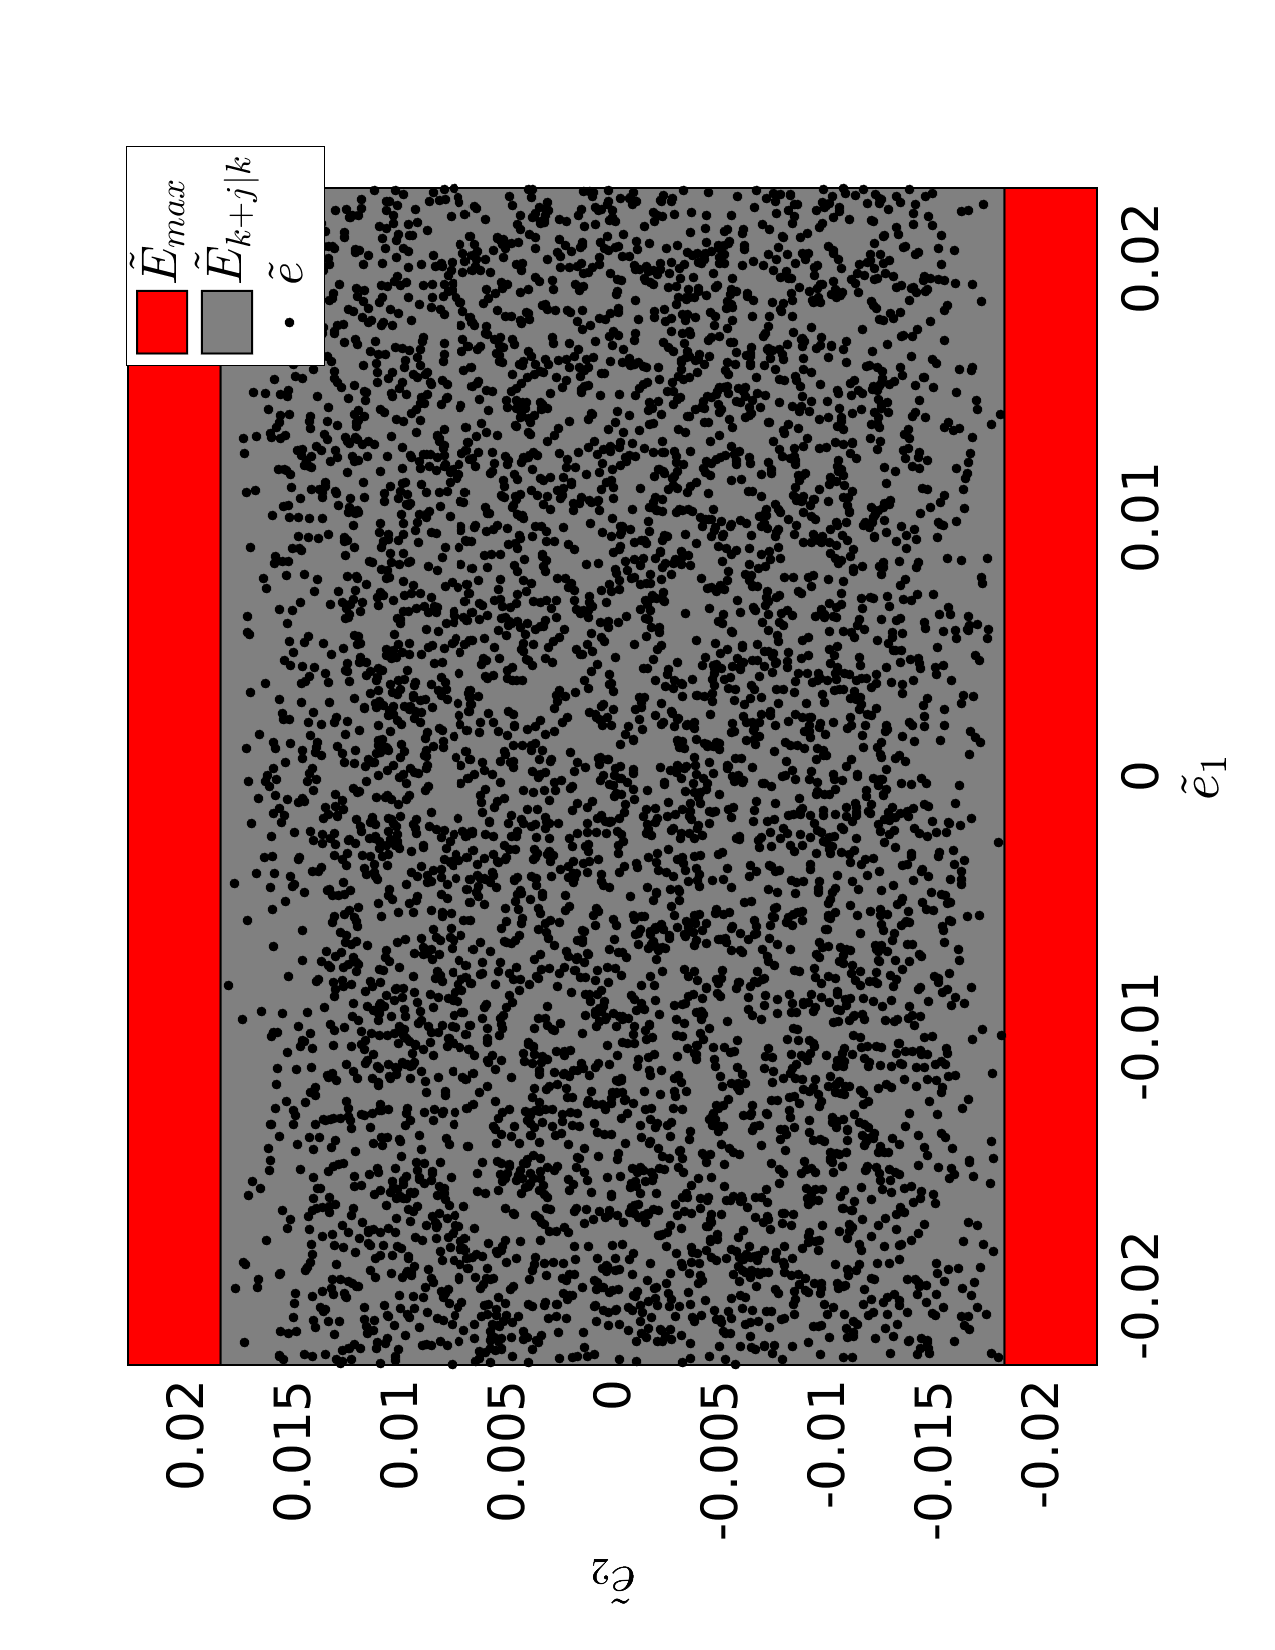
\includegraphics[angle=270,width=0.49\textwidth]{figs/Err_Bounds_toy.pdf}
	\caption{The error sets $\tilde{E}_{max}$ and $\tilde{E}$ computed over an arbitrary $\oa{X}_{k+j|k}$. Also shown are realizations of $\te \defeq T(\hx) - T(x)$ for randomly chosen $x \in \Xc$. Color in online version.}
	\label{fig:err_bound_toy}
\end{figure}

% ====================================
\subsection{Experiments with the Running example}

\begin{figure}
	\centering	
	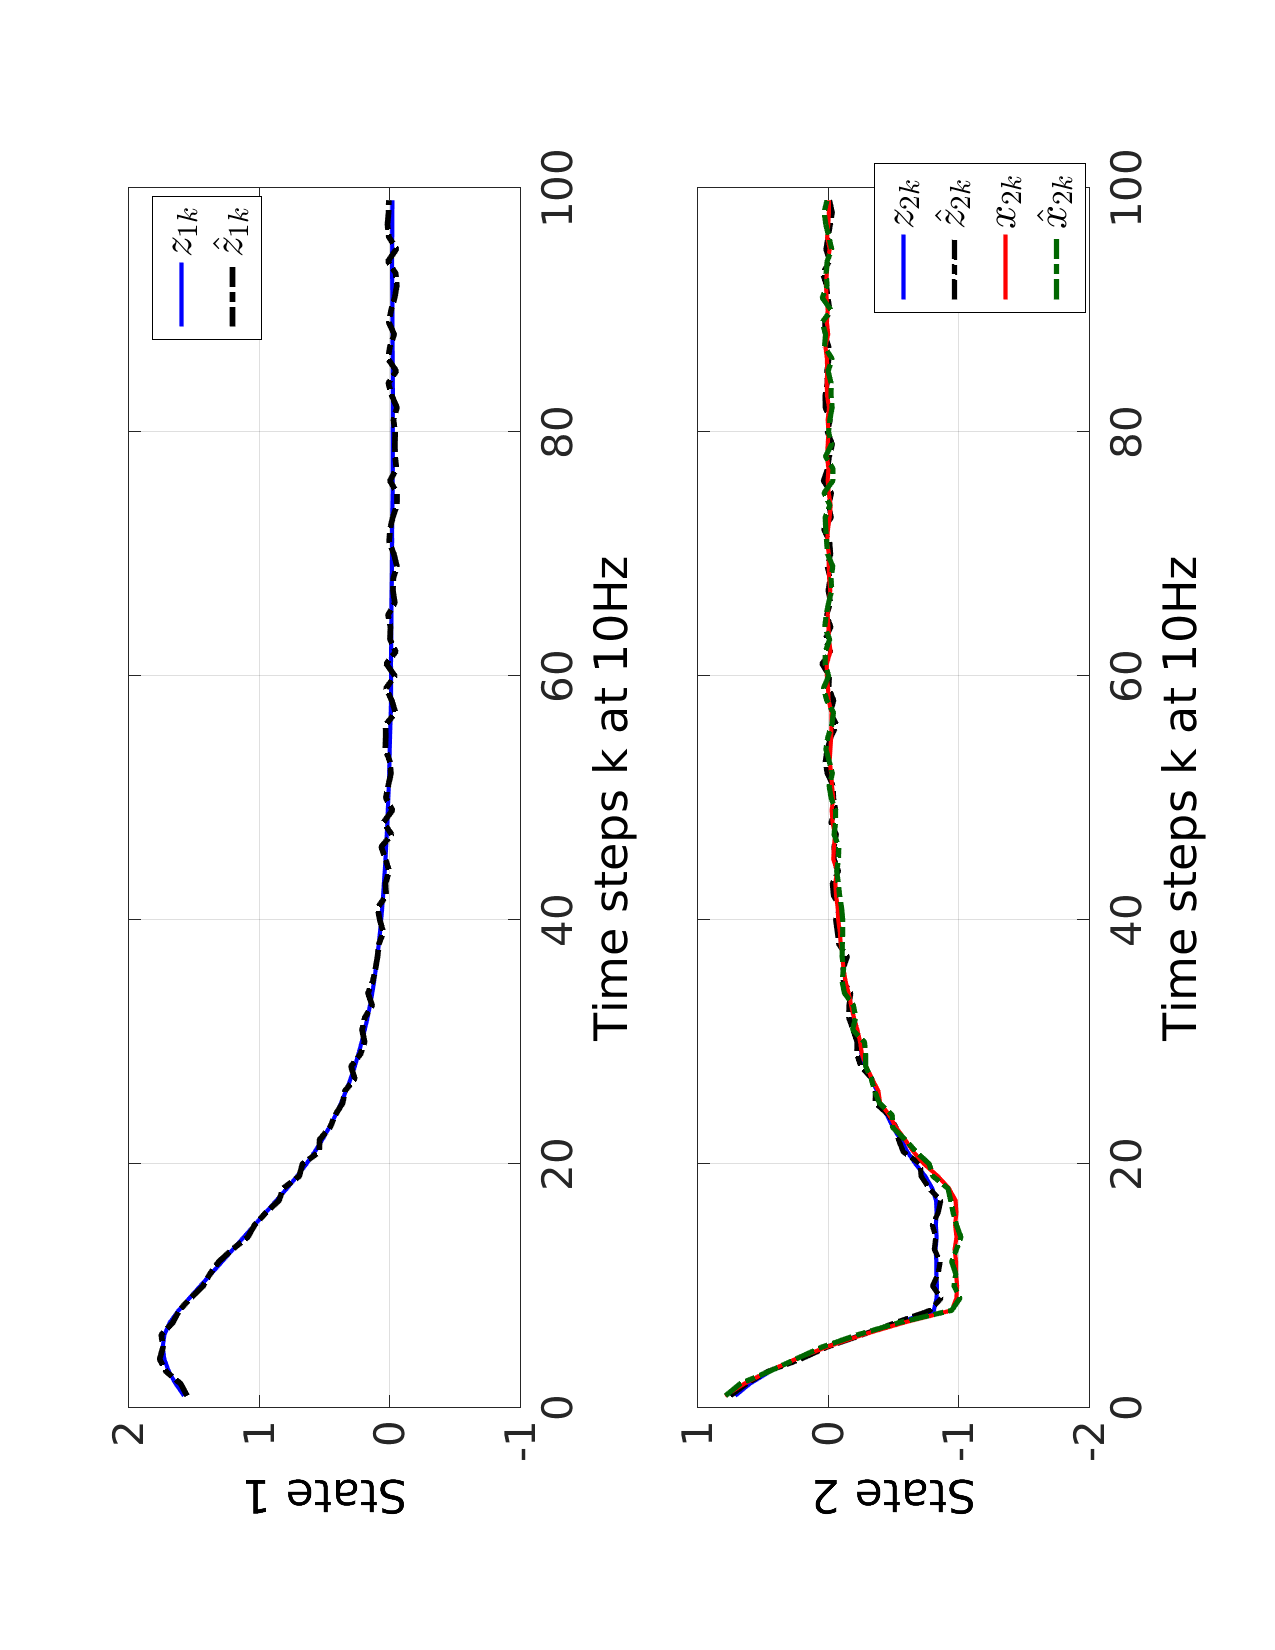
\includegraphics[angle=270,width=0.49\textwidth]{figs/AllStates_toy.pdf}
	\caption{The states and their estimates of the feedback linearized and non-linear running example. Recall that $z_1 = x_1$ therefore to reduce clutter, we only plot the first state only for the feedback linearized system. Color in online version.}
	\label{fig:AllStates_toy}
\end{figure}

For the running example of Eq. \ref{eq:toy_dynamics}, we discretize the feedback linearized system at 10Hz and formulate the controller with a horizon of $N=15$ steps. 
The cost function has parameters $Q=I$ and $R=10^{-2}$, and $W=[-10^{-2}, 10^{-2}]^2$.
The state trajectories (and estimates) for the nonlinear and linearized systems are shown in Fig. \ref{fig:AllStates_toy}.
Note that the states converge to the equilibrium 0. The input $u$ is shown in Fig. \ref{fig:input toy}, and it can be noted that $u_k \in U$ for all $k$.
%(and for the running example, $T$ preserves zero). 

\begin{figure}
	\centering	
	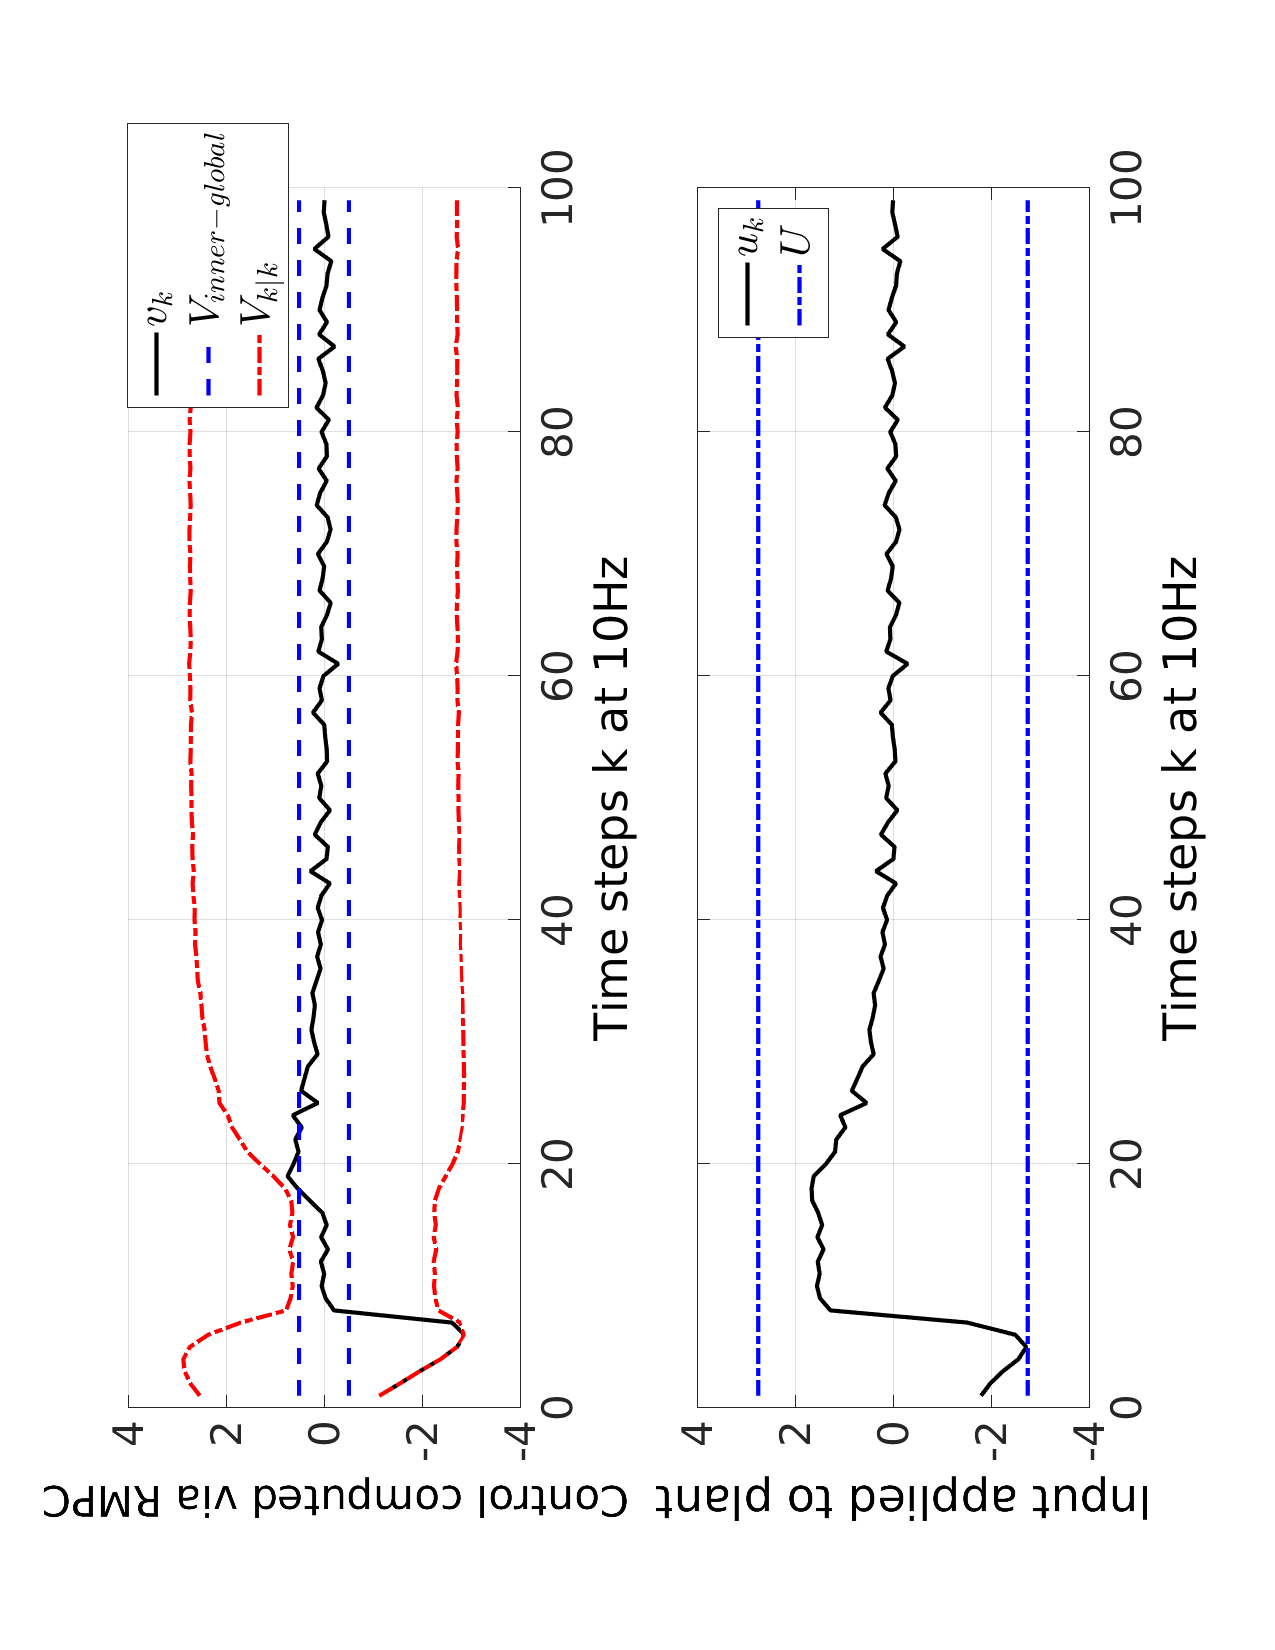
\includegraphics[angle=270,width=0.49\textwidth]{figs/u_and_v_toy.pdf}
	\caption{Inputs $v$ and $u$ and their bounds for the running example. Color in online version.}
	\label{fig:input toy}
\end{figure}


